\documentclass[10pt]{article}

% -------------------- Packages -------------------- %

% Font/input basics
\usepackage[T1]{fontenc}
\usepackage[utf8]{inputenc}
\usepackage{lmodern}

% Critical math packages
\usepackage{amsmath}
\usepackage{amssymb}
\usepackage{mathtools}

% Tools for theorems, including restatement capability
\usepackage{amsthm}
\usepackage{thmtools}
\usepackage{thm-restate}

% Local table of contents capability
\usepackage{etoc}

% General formatting
\usepackage[margin=1in]{geometry}
\usepackage{float}
\usepackage{setspace}
\usepackage{booktabs}
\setcounter{secnumdepth}{0} % No numbered sections
\usepackage[labelsep=period,font=small,labelfont=bf,margin=5ex]{caption}
\usepackage{indentfirst} % Indent first paragraph of sections
%\usepackage[parfill]{parskip} % Remove all indents

% Bibliography and references
\usepackage{multibib}
\usepackage[sort]{natbib}
\usepackage[bookmarks=false]{hyperref}

% -------------------- Setup -------------------- %

% Don't highlight references/links
\hypersetup{
  colorlinks=true,
  citecolor=black,
  linkcolor=black,
  urlcolor=black
}

% Set up natbib
\bibpunct{(}{)}{;}{a}{}{,}  % citations like (Fearon 1995; Powell 1996, 1999)
\def\citeapos#1{\citeauthor{#1}'s (\citeyear{#1})}  % Sartori's (2002)
\renewcommand{\harvardurl}[1]{\textbf{URL:} \url{#1}}  % less-bad URLs in bibliography
\defcitealias{APSA2018}{APSA 2018}
\newcites{app}{Additional References}

% Theorem environments (add more if needed)
\declaretheorem{lemma}
\declaretheorem{corollary}
\declaretheorem{proposition}

% -------------------- Metadata -------------------- %

\title{R Code Appendix for Gill and Zorn, `Debunking the Erroneous Claims of Election Fraud'%
  \thanks{The authors write on behalf of themselves. Nothing in this report should be read as speaking for any institution with which Professor Gill or Professor Zorn are associated. This manuscript is currently under development. Please do not cite this working paper without express permission from the authors.}
}

    \usepackage{authblk}
                                        \author[1]{Rebecca Gill, Ph.D.}
                                                            \affil{University of Nevada Las Vegas \thanks{\href{mailto:rebecca.gill@unlv.edu}{\nolinkurl{rebecca.gill@unlv.edu}}}}
                                                                                \author[2]{Christopher Zorn, Ph.D.}
                                                            \affil{Pennsylvania State University \thanks{\href{mailto:zorn@psu.edu}{\nolinkurl{zorn@psu.edu}}}}
                                            

\usepackage{color}
\usepackage{fancyvrb}
\newcommand{\VerbBar}{|}
\newcommand{\VERB}{\Verb[commandchars=\\\{\}]}
\DefineVerbatimEnvironment{Highlighting}{Verbatim}{commandchars=\\\{\}}
% Add ',fontsize=\small' for more characters per line
\usepackage{framed}
\definecolor{shadecolor}{RGB}{248,248,248}
\newenvironment{Shaded}{\begin{snugshade}}{\end{snugshade}}
\newcommand{\AlertTok}[1]{\textcolor[rgb]{0.94,0.16,0.16}{#1}}
\newcommand{\AnnotationTok}[1]{\textcolor[rgb]{0.56,0.35,0.01}{\textbf{\textit{#1}}}}
\newcommand{\AttributeTok}[1]{\textcolor[rgb]{0.13,0.29,0.53}{#1}}
\newcommand{\BaseNTok}[1]{\textcolor[rgb]{0.00,0.00,0.81}{#1}}
\newcommand{\BuiltInTok}[1]{#1}
\newcommand{\CharTok}[1]{\textcolor[rgb]{0.31,0.60,0.02}{#1}}
\newcommand{\CommentTok}[1]{\textcolor[rgb]{0.56,0.35,0.01}{\textit{#1}}}
\newcommand{\CommentVarTok}[1]{\textcolor[rgb]{0.56,0.35,0.01}{\textbf{\textit{#1}}}}
\newcommand{\ConstantTok}[1]{\textcolor[rgb]{0.56,0.35,0.01}{#1}}
\newcommand{\ControlFlowTok}[1]{\textcolor[rgb]{0.13,0.29,0.53}{\textbf{#1}}}
\newcommand{\DataTypeTok}[1]{\textcolor[rgb]{0.13,0.29,0.53}{#1}}
\newcommand{\DecValTok}[1]{\textcolor[rgb]{0.00,0.00,0.81}{#1}}
\newcommand{\DocumentationTok}[1]{\textcolor[rgb]{0.56,0.35,0.01}{\textbf{\textit{#1}}}}
\newcommand{\ErrorTok}[1]{\textcolor[rgb]{0.64,0.00,0.00}{\textbf{#1}}}
\newcommand{\ExtensionTok}[1]{#1}
\newcommand{\FloatTok}[1]{\textcolor[rgb]{0.00,0.00,0.81}{#1}}
\newcommand{\FunctionTok}[1]{\textcolor[rgb]{0.13,0.29,0.53}{\textbf{#1}}}
\newcommand{\ImportTok}[1]{#1}
\newcommand{\InformationTok}[1]{\textcolor[rgb]{0.56,0.35,0.01}{\textbf{\textit{#1}}}}
\newcommand{\KeywordTok}[1]{\textcolor[rgb]{0.13,0.29,0.53}{\textbf{#1}}}
\newcommand{\NormalTok}[1]{#1}
\newcommand{\OperatorTok}[1]{\textcolor[rgb]{0.81,0.36,0.00}{\textbf{#1}}}
\newcommand{\OtherTok}[1]{\textcolor[rgb]{0.56,0.35,0.01}{#1}}
\newcommand{\PreprocessorTok}[1]{\textcolor[rgb]{0.56,0.35,0.01}{\textit{#1}}}
\newcommand{\RegionMarkerTok}[1]{#1}
\newcommand{\SpecialCharTok}[1]{\textcolor[rgb]{0.81,0.36,0.00}{\textbf{#1}}}
\newcommand{\SpecialStringTok}[1]{\textcolor[rgb]{0.31,0.60,0.02}{#1}}
\newcommand{\StringTok}[1]{\textcolor[rgb]{0.31,0.60,0.02}{#1}}
\newcommand{\VariableTok}[1]{\textcolor[rgb]{0.00,0.00,0.00}{#1}}
\newcommand{\VerbatimStringTok}[1]{\textcolor[rgb]{0.31,0.60,0.02}{#1}}
\newcommand{\WarningTok}[1]{\textcolor[rgb]{0.56,0.35,0.01}{\textbf{\textit{#1}}}}

\thispagestyle{empty}

\begin{document}

% -------------------- Title -------------------- %

\setcounter{page}{0}
\maketitle
\thispagestyle{empty}
\singlespacing

% -------------------- Title -------------------- %

What follows is the R code used to generate the analyses in the original paper.

\begin{Shaded}
\begin{Highlighting}[]
\FunctionTok{library}\NormalTok{(pandoc)}
\FunctionTok{pandoc\_activate}\NormalTok{(}\StringTok{"3.1.6.2"}\NormalTok{, }\AttributeTok{rmarkdown =} \ConstantTok{TRUE}\NormalTok{)}

\FunctionTok{library}\NormalTok{(knitr)}
\FunctionTok{library}\NormalTok{(cowplot)}
\FunctionTok{library}\NormalTok{(olsrr)}
\FunctionTok{library}\NormalTok{(car)}
\FunctionTok{library}\NormalTok{(texreg)}
\FunctionTok{library}\NormalTok{(vtable)}
\FunctionTok{library}\NormalTok{(data.table)                   }
\FunctionTok{library}\NormalTok{(ggeffects)}
\FunctionTok{library}\NormalTok{(GGally)}
\FunctionTok{library}\NormalTok{(datawizard)}
\FunctionTok{library}\NormalTok{(broom)}
\FunctionTok{library}\NormalTok{(tidyverse)}
\end{Highlighting}
\end{Shaded}

\begin{Shaded}
\begin{Highlighting}[]
\NormalTok{cc }\OtherTok{\textless{}{-}} \FunctionTok{fread}\NormalTok{(}
  \StringTok{"https://elections.clarkcountynv.gov/electionresultsTV/sov/20G/PRESIDENT.txt"}\NormalTok{)}

\CommentTok{\# wrangle data}

\NormalTok{candidate\_columns }\OtherTok{\textless{}{-}} \FunctionTok{c}\NormalTok{(}
  \StringTok{"biden"} \OtherTok{=} \StringTok{"Biden, Joseph R."}\NormalTok{,}
  \StringTok{"trump"} \OtherTok{=} \StringTok{"Trump, Donald J."}\NormalTok{,}
  \StringTok{"jorg"}  \OtherTok{=} \StringTok{"Jorgensen, Jo"}\NormalTok{,}
  \StringTok{"blank"} \OtherTok{=}\StringTok{"Blankenship, Don"}\NormalTok{,}
  \StringTok{"none"}  \OtherTok{=} \StringTok{"None of These Candidates"}
\NormalTok{)}

\NormalTok{name\_mapping }\OtherTok{\textless{}{-}} \FunctionTok{c}\NormalTok{(candidate\_columns,}
  \StringTok{"type"}     \OtherTok{=} \StringTok{"Tally Type"}\NormalTok{,}
  \StringTok{"precinct"} \OtherTok{=} \StringTok{"Precinct"}\NormalTok{,}
  \StringTok{"reg"}      \OtherTok{=} \StringTok{"Registration"}\NormalTok{,}
  \StringTok{"turnout"}  \OtherTok{=} \StringTok{"Turnout"}\NormalTok{,}
  \StringTok{"total"}    \OtherTok{=} \StringTok{"Total Votes"}
\NormalTok{)}

\NormalTok{cc }\OtherTok{\textless{}{-}} \FunctionTok{rename}\NormalTok{(cc, }\FunctionTok{all\_of}\NormalTok{(name\_mapping))}

\NormalTok{candidates }\OtherTok{\textless{}{-}} \FunctionTok{c}\NormalTok{(}\StringTok{"biden"}\NormalTok{, }\StringTok{"trump"}\NormalTok{, }\StringTok{"jorg"}\NormalTok{, }\StringTok{"blank"}\NormalTok{, }\StringTok{"none"}\NormalTok{)}

\NormalTok{cc }\OtherTok{\textless{}{-}}\NormalTok{ cc }\SpecialCharTok{\%\textgreater{}\%}
  \FunctionTok{mutate}\NormalTok{(}\FunctionTok{across}\NormalTok{(}\FunctionTok{all\_of}\NormalTok{(candidates), as.numeric))}

\NormalTok{cc }\OtherTok{\textless{}{-}}\NormalTok{ cc }\SpecialCharTok{\%\textgreater{}\%}
  \FunctionTok{mutate}\NormalTok{(}
    \AttributeTok{type =} \FunctionTok{factor}\NormalTok{(type, }
                  \AttributeTok{levels =} \FunctionTok{c}\NormalTok{(}\StringTok{"Totals"}\NormalTok{, }\StringTok{"Election Day"}\NormalTok{, }\StringTok{"Early Vote"}\NormalTok{, }\StringTok{"Mail"}\NormalTok{),}
                  \AttributeTok{labels =} \FunctionTok{c}\NormalTok{(}\StringTok{"totals"}\NormalTok{, }\StringTok{"dayof"}\NormalTok{, }\StringTok{"early"}\NormalTok{, }\StringTok{"mail"}\NormalTok{))}
\NormalTok{  )}

\NormalTok{cc2 }\OtherTok{\textless{}{-}}\NormalTok{ cc }\SpecialCharTok{\%\textgreater{}\%}
  \FunctionTok{filter}\NormalTok{(type }\SpecialCharTok{\%in\%} \FunctionTok{c}\NormalTok{(}\StringTok{"early"}\NormalTok{, }\StringTok{"mail"}\NormalTok{)) }\SpecialCharTok{\%\textgreater{}\%}
  \FunctionTok{select}\NormalTok{(precinct, type, trump, biden) }\SpecialCharTok{\%\textgreater{}\%}
  \FunctionTok{pivot\_wider}\NormalTok{(}\AttributeTok{names\_from =}\NormalTok{ type, }\AttributeTok{values\_from =} \FunctionTok{c}\NormalTok{(trump, biden), }\AttributeTok{names\_sep =} \StringTok{"\_"}\NormalTok{) }\SpecialCharTok{\%\textgreater{}\%}
  \FunctionTok{rename}\NormalTok{(}
    \AttributeTok{t\_e =}\NormalTok{ trump\_early,}
    \AttributeTok{t\_m =}\NormalTok{ trump\_mail,}
    \AttributeTok{b\_e =}\NormalTok{ biden\_early,}
    \AttributeTok{b\_m =}\NormalTok{ biden\_mail}
\NormalTok{  )}

\NormalTok{cc2 }\OtherTok{\textless{}{-}} \FunctionTok{na.omit}\NormalTok{(cc2)}
\FunctionTok{row.names}\NormalTok{(cc2) }\OtherTok{\textless{}{-}} \FunctionTok{as.character}\NormalTok{(cc2}\SpecialCharTok{$}\NormalTok{precinct)}
\FunctionTok{sumtable}\NormalTok{(cc2, }
         \AttributeTok{vars =} \FunctionTok{c}\NormalTok{(}\StringTok{\textquotesingle{}t\_e\textquotesingle{}}\NormalTok{, }\StringTok{\textquotesingle{}t\_m\textquotesingle{}}\NormalTok{, }\StringTok{\textquotesingle{}b\_e\textquotesingle{}}\NormalTok{, }\StringTok{\textquotesingle{}b\_m\textquotesingle{}}\NormalTok{),}
         \AttributeTok{out =} \StringTok{"latex"}\NormalTok{)}
\end{Highlighting}
\end{Shaded}

\begin{table}[!htbp] \centering \renewcommand*{\arraystretch}{1.1}\caption{Summary Statistics}\resizebox{\textwidth}{!}{
\begin{tabular}{lrrrrrrr}
\hline
\hline
Variable & N & Mean & Std. Dev. & Min & Pctl. 25 & Pctl. 75 & Max \\ 
\hline
t\_e & 1065 & 220 & 159 & 0 & 102 & 314 & 1127 \\ 
t\_m & 1065 & 128 & 97 & 0 & 66 & 173 & 844 \\ 
b\_e & 1065 & 161 & 107 & 0 & 93 & 223 & 666 \\ 
b\_m & 1065 & 285 & 175 & 0 & 179 & 386 & 1069\\ 
\hline
\hline
\end{tabular}
}
\end{table}

\begin{Shaded}
\begin{Highlighting}[]
\NormalTok{cc2 }\OtherTok{\textless{}{-}}\NormalTok{ cc2 }\SpecialCharTok{\%\textgreater{}\%}
  \FunctionTok{mutate}\NormalTok{(}\AttributeTok{x =}\NormalTok{ t\_e }\SpecialCharTok{/}\NormalTok{ (t\_e }\SpecialCharTok{+}\NormalTok{ b\_e)) }\SpecialCharTok{\%\textgreater{}\%}
  \FunctionTok{mutate}\NormalTok{(}\AttributeTok{y =}\NormalTok{ t\_m }\SpecialCharTok{/}\NormalTok{ (t\_m }\SpecialCharTok{+}\NormalTok{ b\_m)) }\SpecialCharTok{\%\textgreater{}\%}
  \FunctionTok{mutate}\NormalTok{(}\AttributeTok{g =}\NormalTok{ t\_e }\SpecialCharTok{/}\NormalTok{ (t\_e }\SpecialCharTok{+}\NormalTok{ b\_m)) }\SpecialCharTok{\%\textgreater{}\%}
  \FunctionTok{mutate}\NormalTok{(}\AttributeTok{h =}\NormalTok{ t\_m }\SpecialCharTok{/}\NormalTok{ (t\_m }\SpecialCharTok{+}\NormalTok{ b\_e)) }\SpecialCharTok{\%\textgreater{}\%}
  \FunctionTok{mutate}\NormalTok{(}\AttributeTok{n =}\NormalTok{ t\_e }\SpecialCharTok{+}\NormalTok{ b\_e }\SpecialCharTok{+}\NormalTok{ t\_m }\SpecialCharTok{+}\NormalTok{ b\_m) }\SpecialCharTok{\%\textgreater{}\%}
  \FunctionTok{mutate}\NormalTok{(}\AttributeTok{omega =}\NormalTok{ (t\_e }\SpecialCharTok{+}\NormalTok{ b\_e) }\SpecialCharTok{/}\NormalTok{ n) }\SpecialCharTok{\%\textgreater{}\%}
  \FunctionTok{mutate}\NormalTok{(}\AttributeTok{lambda =}\NormalTok{ (t\_e }\SpecialCharTok{+}\NormalTok{ b\_m) }\SpecialCharTok{/}\NormalTok{ n) }\SpecialCharTok{\%\textgreater{}\%}
  \FunctionTok{mutate}\NormalTok{(}\AttributeTok{alpha =}\NormalTok{ (t\_e }\SpecialCharTok{+}\NormalTok{ t\_m) }\SpecialCharTok{/}\NormalTok{ n)}

\FunctionTok{sumtable}\NormalTok{(cc2, }
         \AttributeTok{vars =} \FunctionTok{c}\NormalTok{(}\StringTok{\textquotesingle{}x\textquotesingle{}}\NormalTok{, }\StringTok{\textquotesingle{}y\textquotesingle{}}\NormalTok{, }\StringTok{\textquotesingle{}g\textquotesingle{}}\NormalTok{, }\StringTok{\textquotesingle{}h\textquotesingle{}}\NormalTok{, }\StringTok{\textquotesingle{}n\textquotesingle{}}\NormalTok{, }\StringTok{\textquotesingle{}omega\textquotesingle{}}\NormalTok{, }\StringTok{\textquotesingle{}lambda\textquotesingle{}}\NormalTok{, }\StringTok{\textquotesingle{}alpha\textquotesingle{}}\NormalTok{),}
         \AttributeTok{out =} \StringTok{\textquotesingle{}latex\textquotesingle{}}\NormalTok{)}
\end{Highlighting}
\end{Shaded}

\begin{table}[!htbp] \centering \renewcommand*{\arraystretch}{1.1}\caption{Summary Statistics}\resizebox{\textwidth}{!}{
\begin{tabular}{lrrrrrrr}
\hline
\hline
Variable & N & Mean & Std. Dev. & Min & Pctl. 25 & Pctl. 75 & Max \\ 
\hline
x & 985 & 0.56 & 0.15 & 0.047 & 0.48 & 0.66 & 1 \\ 
y & 985 & 0.31 & 0.11 & 0.034 & 0.24 & 0.37 & 0.93 \\ 
g & 985 & 0.43 & 0.14 & 0.027 & 0.34 & 0.51 & 0.95 \\ 
h & 985 & 0.45 & 0.15 & 0.043 & 0.35 & 0.52 & 1 \\ 
n & 1065 & 795 & 485 & 0 & 501 & 1069 & 3369 \\ 
omega & 985 & 0.48 & 0.072 & 0.21 & 0.44 & 0.52 & 0.73 \\ 
lambda & 985 & 0.64 & 0.039 & 0.41 & 0.61 & 0.66 & 0.82 \\ 
alpha & 985 & 0.43 & 0.13 & 0.052 & 0.35 & 0.51 & 0.96\\ 
\hline
\hline
\end{tabular}
}
\end{table}

\begin{Shaded}
\begin{Highlighting}[]
\NormalTok{std.fit }\OtherTok{\textless{}{-}} \FunctionTok{lm}\NormalTok{(alpha }\SpecialCharTok{\textasciitilde{}}\NormalTok{ y }\SpecialCharTok{+}\NormalTok{ x, }\AttributeTok{data =}\NormalTok{ cc2)}
\NormalTok{bst.fit }\OtherTok{\textless{}{-}} \FunctionTok{lm}\NormalTok{(alpha }\SpecialCharTok{\textasciitilde{}}\NormalTok{ g }\SpecialCharTok{+}\NormalTok{ h, }\AttributeTok{data =}\NormalTok{ cc2)}

\FunctionTok{texreg}\NormalTok{(}\FunctionTok{list}\NormalTok{(std.fit, bst.fit),}
       \AttributeTok{custom.model.names =} \FunctionTok{c}\NormalTok{(}\StringTok{"Standard"}\NormalTok{, }\StringTok{"Bastard"}\NormalTok{),}
       \AttributeTok{caption.above =} \ConstantTok{TRUE}\NormalTok{)}
\end{Highlighting}
\end{Shaded}

\begin{table}
\caption{Statistical models}
\begin{center}
\begin{tabular}{l c c}
\hline
 & Standard & Bastard \\
\hline
(Intercept) & $-0.02^{***}$ & $-0.00^{**}$ \\
            & $(0.00)$      & $(0.00)$     \\
y           & $0.49^{***}$  &              \\
            & $(0.01)$      &              \\
x           & $0.53^{***}$  &              \\
            & $(0.01)$      &              \\
g           &               & $0.64^{***}$ \\
            &               & $(0.00)$     \\
h           &               & $0.37^{***}$ \\
            &               & $(0.00)$     \\
\hline
R$^2$       & $0.98$        & $1.00$       \\
Adj. R$^2$  & $0.98$        & $1.00$       \\
Num. obs.   & $985$         & $985$        \\
\hline
\multicolumn{3}{l}{\scriptsize{$^{***}p<0.001$; $^{**}p<0.01$; $^{*}p<0.05$}}
\end{tabular}
\label{table:coefficients}
\end{center}
\end{table}

\begin{Shaded}
\begin{Highlighting}[]
\NormalTok{std.prd }\OtherTok{\textless{}{-}} \FunctionTok{ggpredict}\NormalTok{(std.fit, }\AttributeTok{terms =} \FunctionTok{c}\NormalTok{(}\StringTok{"y"}\NormalTok{, }\StringTok{"x"}\NormalTok{))}
\NormalTok{std.plt }\OtherTok{\textless{}{-}} \FunctionTok{plot}\NormalTok{(std.prd) }

\NormalTok{bst.prd }\OtherTok{\textless{}{-}} \FunctionTok{ggpredict}\NormalTok{(bst.fit, }\AttributeTok{terms =} \FunctionTok{c}\NormalTok{(}\StringTok{"g"}\NormalTok{, }\StringTok{"h"}\NormalTok{))}
\NormalTok{bst.plt }\OtherTok{\textless{}{-}} \FunctionTok{plot}\NormalTok{(bst.prd)}

\FunctionTok{plot\_grid}\NormalTok{(std.plt, bst.plt)}
\end{Highlighting}
\end{Shaded}

\begin{figure}
\centering
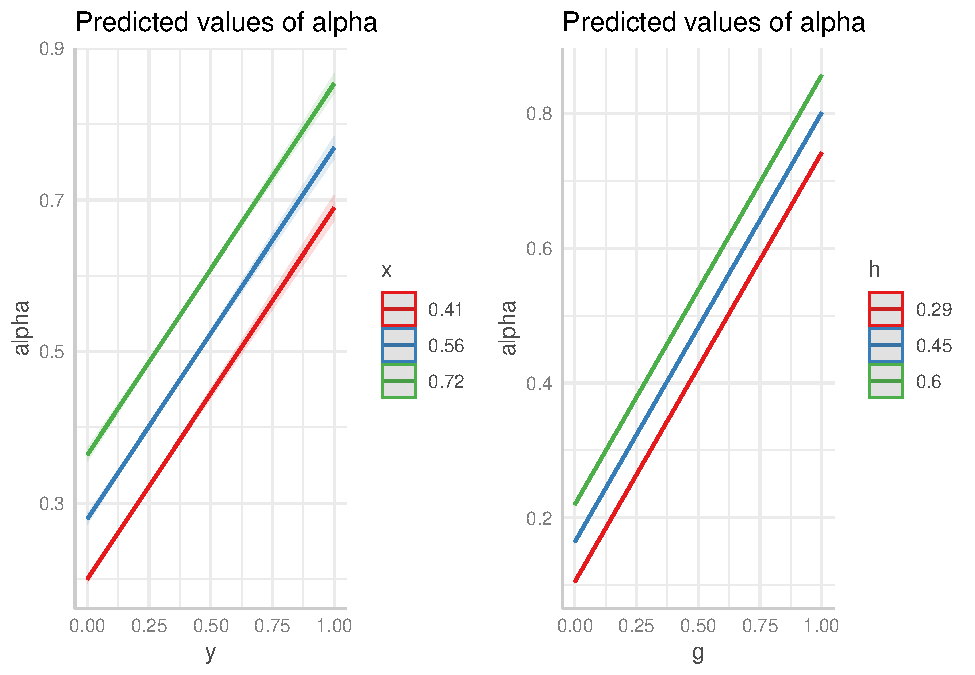
\includegraphics{CodeAppendix_files/figure-latex/figz2-1.pdf}
\caption{\label{fig:figz2}Predicted Values of Trump Vote Share}
\end{figure}

\begin{Shaded}
\begin{Highlighting}[]
\NormalTok{wc }\OtherTok{\textless{}{-}} \FunctionTok{read\_csv}\NormalTok{(}\StringTok{"rawdata/Washoe.csv"}\NormalTok{)}

\CommentTok{\# wrangle}

\NormalTok{reno5 }\OtherTok{\textless{}{-}}\NormalTok{ wc }\SpecialCharTok{\%\textgreater{}\%} \CommentTok{\# select variables}
  \FunctionTok{select}\NormalTok{(PrecinctPortion, CountingGroup,}
         \FunctionTok{starts\_with}\NormalTok{(}\StringTok{"RENO.CITY.COUNCIL..WARD.5"}\NormalTok{))}

\NormalTok{candidate\_columns }\OtherTok{\textless{}{-}} \FunctionTok{c}\NormalTok{( }\CommentTok{\# candidate vars to rename}
  \StringTok{"sbp"} \OtherTok{=} \StringTok{"RENO.CITY.COUNCIL..WARD.5..Vote.For.1.\_BROWNING.PEUCHAUD..SHEILA\_NP"}\NormalTok{,}
  \StringTok{"bmc"} \OtherTok{=} \StringTok{"RENO.CITY.COUNCIL..WARD.5..Vote.For.1.\_CASSIDY..BRIAN.M.\_NP"}\NormalTok{,}
  \StringTok{"dtr"} \OtherTok{=} \StringTok{"RENO.CITY.COUNCIL..WARD.5..Vote.For.1.\_REESE..DEVON.T.\_NP"}\NormalTok{,}
  \StringTok{"tcw"} \OtherTok{=} \StringTok{"RENO.CITY.COUNCIL..WARD.5..Vote.For.1.\_WEBSTER..TARA.C.\_NP"}
\NormalTok{)}

\NormalTok{name\_mapping }\OtherTok{\textless{}{-}} \FunctionTok{c}\NormalTok{(candidate\_columns, }\CommentTok{\# all vars to rename}
  \StringTok{"precinct"} \OtherTok{=} \StringTok{"PrecinctPortion"}\NormalTok{,}
  \StringTok{"type"}     \OtherTok{=} \StringTok{"CountingGroup"}
\NormalTok{)}

\NormalTok{reno5 }\OtherTok{\textless{}{-}} \FunctionTok{rename}\NormalTok{(reno5, }\FunctionTok{all\_of}\NormalTok{(name\_mapping)) }\CommentTok{\# rename them}

\NormalTok{candidates }\OtherTok{\textless{}{-}} \FunctionTok{c}\NormalTok{(}\StringTok{"sbp"}\NormalTok{, }\StringTok{"bmc"}\NormalTok{, }\StringTok{"dtr"}\NormalTok{, }\StringTok{"tcw"}\NormalTok{) }\CommentTok{\# new list of candidates}

\NormalTok{reno5 }\OtherTok{\textless{}{-}}\NormalTok{ reno5 }\SpecialCharTok{\%\textgreater{}\%} \CommentTok{\# fix the precinct var and drop obs from other wards}
  \FunctionTok{mutate}\NormalTok{(}\FunctionTok{across}\NormalTok{(}\FunctionTok{all\_of}\NormalTok{(candidates), as.numeric)) }\SpecialCharTok{\%\textgreater{}\%}
  \FunctionTok{drop\_na}\NormalTok{(}\FunctionTok{all\_of}\NormalTok{(candidates)) }\SpecialCharTok{\%\textgreater{}\%}
  \FunctionTok{mutate}\NormalTok{(}\AttributeTok{precinct =} \FunctionTok{str\_extract}\NormalTok{(precinct, }\StringTok{"}\SpecialCharTok{\textbackslash{}\textbackslash{}}\StringTok{((}\SpecialCharTok{\textbackslash{}\textbackslash{}}\StringTok{d+)}\SpecialCharTok{\textbackslash{}\textbackslash{}}\StringTok{)"}\NormalTok{)) }\SpecialCharTok{\%\textgreater{}\%}
  \FunctionTok{mutate}\NormalTok{(}\AttributeTok{precinct =} \FunctionTok{factor}\NormalTok{(}\FunctionTok{str\_replace\_all}\NormalTok{(precinct, }\StringTok{"[()]"}\NormalTok{, }\StringTok{""}\NormalTok{)))}

\NormalTok{reno5 }\OtherTok{\textless{}{-}}\NormalTok{ reno5 }\SpecialCharTok{\%\textgreater{}\%} \CommentTok{\# fix the type variable}
  \FunctionTok{mutate}\NormalTok{(}
    \AttributeTok{type =} \FunctionTok{factor}\NormalTok{(type, }
                  \AttributeTok{levels =} \FunctionTok{c}\NormalTok{(}\StringTok{"Early Voting"}\NormalTok{, }\StringTok{"Election Day"}\NormalTok{, }\StringTok{"Mail"}\NormalTok{),}
                  \AttributeTok{labels =} \FunctionTok{c}\NormalTok{(}\StringTok{"early"}\NormalTok{, }\StringTok{"dayof"}\NormalTok{, }\StringTok{"mail"}\NormalTok{))}
\NormalTok{  )}

\NormalTok{reno5.sum }\OtherTok{\textless{}{-}}\NormalTok{ reno5 }\SpecialCharTok{\%\textgreater{}\%} \CommentTok{\# make summary}
  \FunctionTok{group\_by}\NormalTok{(precinct, type) }\SpecialCharTok{\%\textgreater{}\%}
  \FunctionTok{summarize}\NormalTok{(}\FunctionTok{across}\NormalTok{(}\FunctionTok{c}\NormalTok{(sbp, bmc, dtr, tcw), }
\NormalTok{                   sum, }
                   \AttributeTok{na.rm =} \ConstantTok{TRUE}\NormalTok{), }
            \AttributeTok{.groups =} \StringTok{\textquotesingle{}drop\textquotesingle{}}\NormalTok{)}

\NormalTok{reno5.wide }\OtherTok{\textless{}{-}}\NormalTok{ reno5.sum }\SpecialCharTok{\%\textgreater{}\%}
  \FunctionTok{pivot\_wider}\NormalTok{(}\AttributeTok{names\_from =}\NormalTok{ type, }
              \AttributeTok{values\_from =} \FunctionTok{c}\NormalTok{(sbp, bmc, dtr, tcw), }
              \AttributeTok{names\_sep =} \StringTok{"\_"}\NormalTok{)}

\NormalTok{labz }\OtherTok{\textless{}{-}} \FunctionTok{c}\NormalTok{(}\StringTok{\textquotesingle{}SBP Early Vote\textquotesingle{}}\NormalTok{, }\StringTok{\textquotesingle{}SBP Election Day\textquotesingle{}}\NormalTok{, }\StringTok{\textquotesingle{}SBP Mail\textquotesingle{}}\NormalTok{,}
          \StringTok{\textquotesingle{}BMC Early Vote\textquotesingle{}}\NormalTok{, }\StringTok{\textquotesingle{}BMC Election Day\textquotesingle{}}\NormalTok{, }\StringTok{\textquotesingle{}BMC Mail\textquotesingle{}}\NormalTok{,}
          \StringTok{\textquotesingle{}DTR Early Vote\textquotesingle{}}\NormalTok{, }\StringTok{\textquotesingle{}DTR Election Day\textquotesingle{}}\NormalTok{, }\StringTok{\textquotesingle{}DTR Mail\textquotesingle{}}\NormalTok{,}
          \StringTok{\textquotesingle{}TCW Early Vote\textquotesingle{}}\NormalTok{, }\StringTok{\textquotesingle{}TCW Election Day\textquotesingle{}}\NormalTok{, }\StringTok{\textquotesingle{}TCW Mail\textquotesingle{}}\NormalTok{)}

\NormalTok{reno5.sm }\OtherTok{\textless{}{-}} \FunctionTok{na.omit}\NormalTok{(reno5.wide) }\CommentTok{\# drop the NAs}
\NormalTok{reno5.sm }\OtherTok{\textless{}{-}}\NormalTok{ reno5.sm[}\SpecialCharTok{{-}}\DecValTok{2}\NormalTok{,] }\CommentTok{\# drop the NAN }

\FunctionTok{sumtable}\NormalTok{(reno5.sm, }
         \AttributeTok{vars =} \FunctionTok{c}\NormalTok{(}\StringTok{\textquotesingle{}sbp\_early\textquotesingle{}}\NormalTok{, }\StringTok{\textquotesingle{}sbp\_dayof\textquotesingle{}}\NormalTok{, }\StringTok{\textquotesingle{}sbp\_mail\textquotesingle{}}\NormalTok{,}
                  \StringTok{\textquotesingle{}bmc\_early\textquotesingle{}}\NormalTok{, }\StringTok{\textquotesingle{}bmc\_dayof\textquotesingle{}}\NormalTok{, }\StringTok{\textquotesingle{}bmc\_mail\textquotesingle{}}\NormalTok{,}
                  \StringTok{\textquotesingle{}dtr\_early\textquotesingle{}}\NormalTok{, }\StringTok{\textquotesingle{}dtr\_dayof\textquotesingle{}}\NormalTok{, }\StringTok{\textquotesingle{}dtr\_mail\textquotesingle{}}\NormalTok{,}
                  \StringTok{\textquotesingle{}tcw\_early\textquotesingle{}}\NormalTok{, }\StringTok{\textquotesingle{}tcw\_dayof\textquotesingle{}}\NormalTok{, }\StringTok{\textquotesingle{}tcw\_mail\textquotesingle{}}\NormalTok{),}
         \AttributeTok{labels =}\NormalTok{ labz,}
         \AttributeTok{out =} \StringTok{"latex"}\NormalTok{)}
\end{Highlighting}
\end{Shaded}

\begin{table}[!htbp] \centering \renewcommand*{\arraystretch}{1.1}\caption{Summary Statistics}\resizebox{\textwidth}{!}{
\begin{tabular}{lrrrrrrr}
\hline
\hline
Variable & N & Mean & Std. Dev. & Min & Pctl. 25 & Pctl. 75 & Max \\ 
\hline
SBP Early Vote & 16 & 9.9 & 6.8 & 0 & 5 & 15 & 21 \\ 
SBP Election Day & 16 & 12 & 6.9 & 1 & 8.5 & 15 & 24 \\ 
SBP Mail & 16 & 79 & 68 & 1 & 42 & 92 & 267 \\ 
BMC Early Vote & 16 & 22 & 15 & 1 & 11 & 35 & 44 \\ 
BMC Election Day & 16 & 31 & 20 & 0 & 21 & 41 & 79 \\ 
BMC Mail & 16 & 99 & 102 & 1 & 43 & 107 & 390 \\ 
DTR Early Vote & 16 & 24 & 17 & 0 & 12 & 36 & 54 \\ 
DTR Election Day & 16 & 26 & 16 & 1 & 16 & 38 & 48 \\ 
DTR Mail & 16 & 156 & 106 & 1 & 86 & 208 & 402 \\ 
TCW Early Vote & 16 & 8.9 & 7 & 0 & 2.5 & 14 & 21 \\ 
TCW Election Day & 16 & 13 & 9 & 0 & 7 & 19 & 30 \\ 
TCW Mail & 16 & 74 & 48 & 0 & 38 & 108 & 149\\ 
\hline
\hline
\end{tabular}
}
\end{table}

\begin{Shaded}
\begin{Highlighting}[]
\NormalTok{reno5.sm }\OtherTok{\textless{}{-}}\NormalTok{ reno5.sm }\SpecialCharTok{\%\textgreater{}\%}
  \FunctionTok{mutate}\NormalTok{(}\AttributeTok{A =}\NormalTok{ bmc\_early }\SpecialCharTok{+}\NormalTok{ bmc\_dayof }\SpecialCharTok{+}\NormalTok{ sbp\_dayof) }\SpecialCharTok{\%\textgreater{}\%}
  \FunctionTok{mutate}\NormalTok{(}\AttributeTok{B =}\NormalTok{ dtr\_early }\SpecialCharTok{+}\NormalTok{ dtr\_dayof }\SpecialCharTok{+}\NormalTok{ bmc\_mail) }\SpecialCharTok{\%\textgreater{}\%}
  \FunctionTok{mutate}\NormalTok{(}\AttributeTok{C =}\NormalTok{ tcw\_mail) }\SpecialCharTok{\%\textgreater{}\%}
  \FunctionTok{mutate}\NormalTok{(}\AttributeTok{D =}\NormalTok{ dtr\_mail }\SpecialCharTok{+}\NormalTok{ sbp\_mail) }\SpecialCharTok{\%\textgreater{}\%}
  \FunctionTok{mutate}\NormalTok{(}\AttributeTok{n =}\NormalTok{ A }\SpecialCharTok{+}\NormalTok{ B }\SpecialCharTok{+}\NormalTok{ C }\SpecialCharTok{+}\NormalTok{ D) }\SpecialCharTok{\%\textgreater{}\%}
  \FunctionTok{mutate}\NormalTok{(}\AttributeTok{g =}\NormalTok{ A }\SpecialCharTok{/}\NormalTok{ (A }\SpecialCharTok{+}\NormalTok{ D)) }\SpecialCharTok{\%\textgreater{}\%}
  \FunctionTok{mutate}\NormalTok{(}\AttributeTok{h =}\NormalTok{ C }\SpecialCharTok{/}\NormalTok{ (C }\SpecialCharTok{+}\NormalTok{ B)) }\SpecialCharTok{\%\textgreater{}\%}
  \FunctionTok{mutate}\NormalTok{(}\AttributeTok{lambda =}\NormalTok{ (A }\SpecialCharTok{+}\NormalTok{ D) }\SpecialCharTok{/}\NormalTok{ n) }\SpecialCharTok{\%\textgreater{}\%}
  \FunctionTok{mutate}\NormalTok{(}\AttributeTok{alpha =}\NormalTok{ (A }\SpecialCharTok{+}\NormalTok{ C) }\SpecialCharTok{/}\NormalTok{ n)}

\FunctionTok{sumtable}\NormalTok{(reno5.sm, }
         \AttributeTok{vars =} \FunctionTok{c}\NormalTok{(}\StringTok{\textquotesingle{}A\textquotesingle{}}\NormalTok{, }\StringTok{\textquotesingle{}B\textquotesingle{}}\NormalTok{, }\StringTok{\textquotesingle{}C\textquotesingle{}}\NormalTok{, }\StringTok{\textquotesingle{}D\textquotesingle{}}\NormalTok{, }\StringTok{\textquotesingle{}n\textquotesingle{}}\NormalTok{, }\StringTok{\textquotesingle{}g\textquotesingle{}}\NormalTok{, }\StringTok{\textquotesingle{}h\textquotesingle{}}\NormalTok{,}\StringTok{\textquotesingle{}lambda\textquotesingle{}}\NormalTok{, }\StringTok{\textquotesingle{}alpha\textquotesingle{}}\NormalTok{),}
         \AttributeTok{out =} \StringTok{\textquotesingle{}latex\textquotesingle{}}\NormalTok{)}
\end{Highlighting}
\end{Shaded}

\begin{table}[!htbp] \centering \renewcommand*{\arraystretch}{1.1}\caption{Summary Statistics}\resizebox{\textwidth}{!}{
\begin{tabular}{lrrrrrrr}
\hline
\hline
Variable & N & Mean & Std. Dev. & Min & Pctl. 25 & Pctl. 75 & Max \\ 
\hline
A & 16 & 65 & 39 & 2 & 42 & 88 & 141 \\ 
B & 16 & 149 & 119 & 5 & 83 & 190 & 451 \\ 
C & 16 & 74 & 48 & 0 & 38 & 108 & 149 \\ 
D & 16 & 235 & 169 & 3 & 128 & 292 & 669 \\ 
n & 16 & 523 & 353 & 12 & 311 & 646 & 1368 \\ 
g & 16 & 0.26 & 0.14 & 0.13 & 0.21 & 0.24 & 0.75 \\ 
h & 16 & 0.3 & 0.18 & 0 & 0.17 & 0.42 & 0.56 \\ 
lambda & 16 & 0.57 & 0.027 & 0.52 & 0.56 & 0.59 & 0.63 \\ 
alpha & 16 & 0.28 & 0.087 & 0.17 & 0.19 & 0.34 & 0.47\\ 
\hline
\hline
\end{tabular}
}
\end{table}

\begin{Shaded}
\begin{Highlighting}[]
\NormalTok{reno.fit }\OtherTok{\textless{}{-}} \FunctionTok{lm}\NormalTok{(alpha }\SpecialCharTok{\textasciitilde{}}\NormalTok{ g }\SpecialCharTok{+}\NormalTok{ h, }\AttributeTok{data =}\NormalTok{ reno5.sm)}
\NormalTok{reno3.fit }\OtherTok{\textless{}{-}} \FunctionTok{lm}\NormalTok{(alpha }\SpecialCharTok{\textasciitilde{}}\NormalTok{ g }\SpecialCharTok{+} \FunctionTok{poly}\NormalTok{(h, }\DecValTok{3}\NormalTok{), }\AttributeTok{data =}\NormalTok{ reno5.sm)}
\FunctionTok{texreg}\NormalTok{(}\FunctionTok{list}\NormalTok{(reno.fit, reno3.fit),}
       \AttributeTok{custom.model.names =} \FunctionTok{c}\NormalTok{(}\StringTok{"Bastard Model"}\NormalTok{, }\StringTok{"Bastard Cubic Model"}\NormalTok{),}
       \AttributeTok{caption.above =} \ConstantTok{TRUE}\NormalTok{)}
\end{Highlighting}
\end{Shaded}

\begin{table}
\caption{Statistical models}
\begin{center}
\begin{tabular}{l c c}
\hline
 & Bastard Model & Bastard Cubic Model \\
\hline
(Intercept) & $-0.02^{**}$ & $0.11^{***}$ \\
            & $(0.01)$     & $(0.00)$     \\
g           & $0.66^{***}$ & $0.65^{***}$ \\
            & $(0.01)$     & $(0.02)$     \\
h           & $0.44^{***}$ &              \\
            & $(0.01)$     &              \\
poly(h, 3)1 &              & $0.31^{***}$ \\
            &              & $(0.01)$     \\
poly(h, 3)2 &              & $0.01$       \\
            &              & $(0.01)$     \\
poly(h, 3)3 &              & $0.01$       \\
            &              & $(0.01)$     \\
\hline
R$^2$       & $1.00$       & $1.00$       \\
Adj. R$^2$  & $0.99$       & $1.00$       \\
Num. obs.   & $16$         & $16$         \\
\hline
\multicolumn{3}{l}{\scriptsize{$^{***}p<0.001$; $^{**}p<0.01$; $^{*}p<0.05$}}
\end{tabular}
\label{table:coefficients}
\end{center}
\end{table}

\begin{Shaded}
\begin{Highlighting}[]
\NormalTok{omega.hist }\OtherTok{\textless{}{-}} \FunctionTok{ggplot}\NormalTok{(cc2, }\FunctionTok{aes}\NormalTok{(}\AttributeTok{x =}\NormalTok{ omega)) }\SpecialCharTok{+}
  \FunctionTok{geom\_histogram}\NormalTok{(}\AttributeTok{fill =} \StringTok{"cornflowerblue"}\NormalTok{, }
                 \AttributeTok{color =} \StringTok{"black"}\NormalTok{) }\SpecialCharTok{+} 
  \FunctionTok{labs}\NormalTok{(}\AttributeTok{title=}\StringTok{"Distribution of Omega"}\NormalTok{,}
       \AttributeTok{x =} \StringTok{"Omega"}\NormalTok{) }

\NormalTok{lambda.hist }\OtherTok{\textless{}{-}} \FunctionTok{ggplot}\NormalTok{(cc2, }\FunctionTok{aes}\NormalTok{(}\AttributeTok{x =}\NormalTok{ lambda)) }\SpecialCharTok{+}
  \FunctionTok{geom\_histogram}\NormalTok{(}\AttributeTok{fill =} \StringTok{"firebrick"}\NormalTok{, }
                 \AttributeTok{color =} \StringTok{"black"}\NormalTok{) }\SpecialCharTok{+} 
  \FunctionTok{labs}\NormalTok{(}\AttributeTok{title=}\StringTok{"Distribution of Lambda"}\NormalTok{,}
       \AttributeTok{x =} \StringTok{"Lambda"}\NormalTok{)}

\FunctionTok{plot\_grid}\NormalTok{(omega.hist, lambda.hist)}
\end{Highlighting}
\end{Shaded}

\begin{figure}
\centering
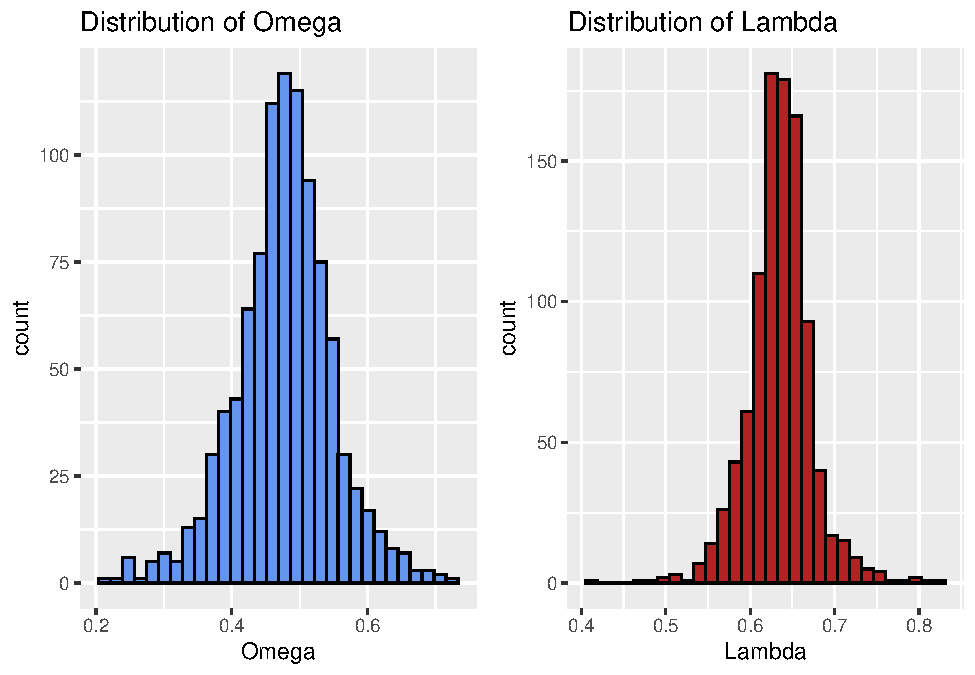
\includegraphics{CodeAppendix_files/figure-latex/hists1-1.pdf}
\caption{\label{fig:hists1}Distribution of Omega and Lambda (Calculated)}
\end{figure}

\begin{Shaded}
\begin{Highlighting}[]
\NormalTok{cc2 }\OtherTok{\textless{}{-}} \FunctionTok{augment}\NormalTok{(bst.fit) }\CommentTok{\# put resids into data frame}
\NormalTok{cc2}\SpecialCharTok{$}\NormalTok{dist0 }\OtherTok{\textless{}{-}} \FunctionTok{abs}\NormalTok{(cc2}\SpecialCharTok{$}\NormalTok{.resid) }\CommentTok{\# calculate error magnitude}

\FunctionTok{ggplot}\NormalTok{(cc2, }\FunctionTok{aes}\NormalTok{(}\AttributeTok{x =}\NormalTok{ .fitted, }\AttributeTok{y =}\NormalTok{ .resid, }\AttributeTok{color =}\NormalTok{ dist0)) }\SpecialCharTok{+}
  \FunctionTok{geom\_point}\NormalTok{() }\SpecialCharTok{+}
  \FunctionTok{scale\_color\_gradient}\NormalTok{(}\AttributeTok{low =} \StringTok{"cornflowerblue"}\NormalTok{, }\AttributeTok{high =} \StringTok{"firebrick"}\NormalTok{) }\SpecialCharTok{+}
  \FunctionTok{labs}\NormalTok{(}\AttributeTok{color =} \StringTok{"Error Size"}\NormalTok{) }\SpecialCharTok{+}
  \FunctionTok{xlab}\NormalTok{(}\StringTok{"Predicted Alpha"}\NormalTok{) }\SpecialCharTok{+}
  \FunctionTok{ylab}\NormalTok{(}\StringTok{"Residual"}\NormalTok{) }\SpecialCharTok{+}
  \FunctionTok{theme\_minimal}\NormalTok{() }\SpecialCharTok{+}
  \FunctionTok{theme}\NormalTok{(}\AttributeTok{legend.position =} \StringTok{"right"}\NormalTok{)}
\end{Highlighting}
\end{Shaded}

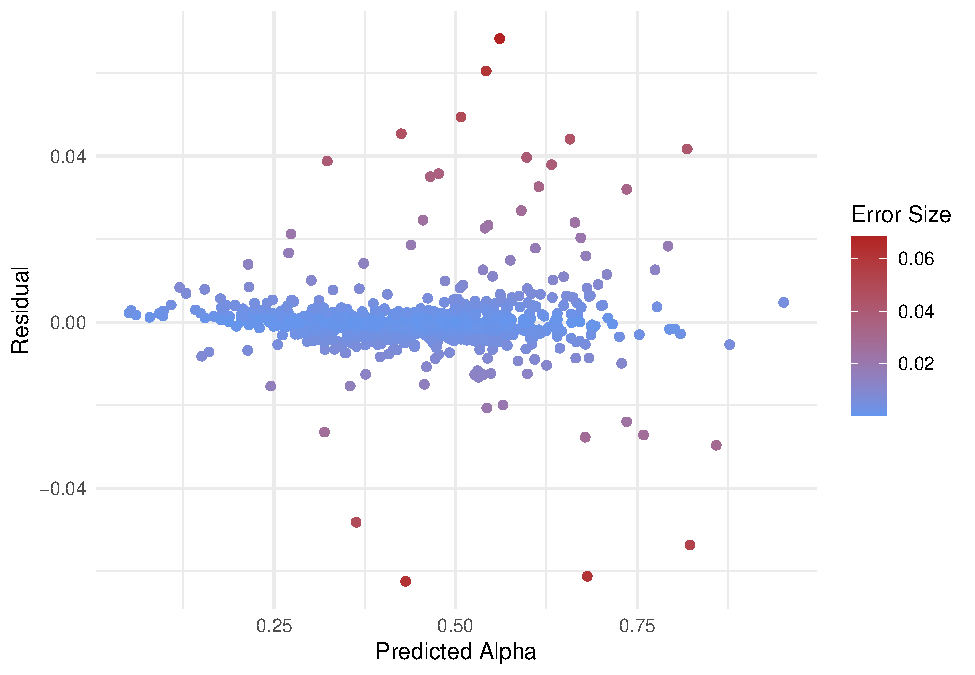
\includegraphics{CodeAppendix_files/figure-latex/residz-1.pdf}

\begin{Shaded}
\begin{Highlighting}[]
\FunctionTok{influencePlot}\NormalTok{(bst.fit)}
\end{Highlighting}
\end{Shaded}

\begin{figure}
\centering
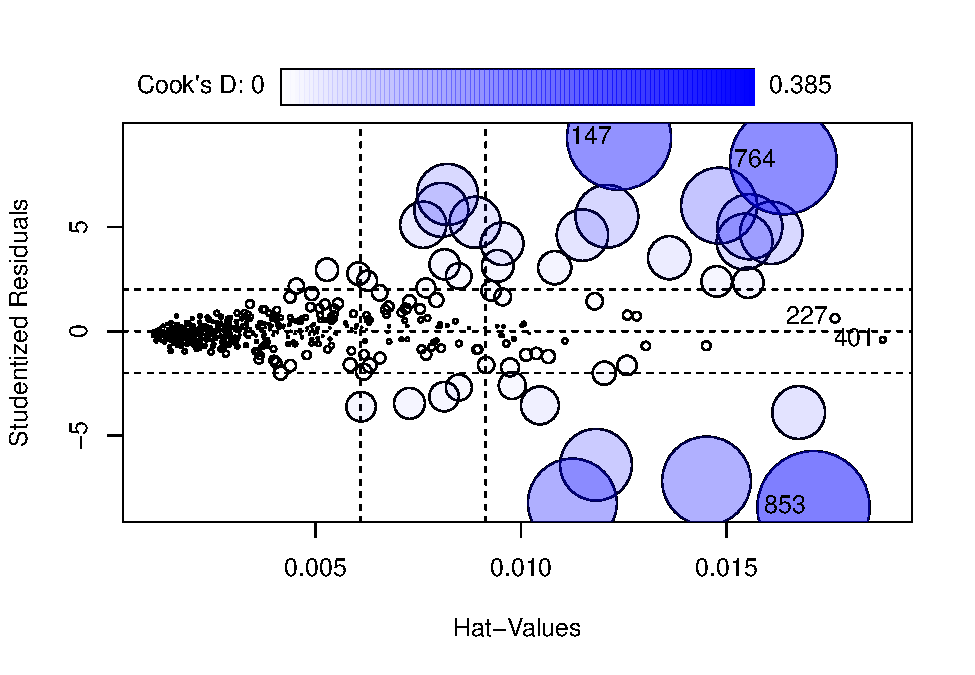
\includegraphics{CodeAppendix_files/figure-latex/infl-1.pdf}
\caption{\label{fig:infl}Influence of Outliers on Lambda Estimate}
\end{figure}

\singlespacing
\newpage
\bibliographystyleapp{apsa-leeper}
\bibliographyapp{references}

\end{document}
